\section{Virtual Memory*}
\subsection{Problem Space}
\noindent
This section is a quick aside to understand the problem we are going 
to solve in the next section when we talk about distributing shared memory \cite{virtualmemory2023}. Virtual memory solves three core problems:
\begin{itemize}
    \item \textbf{Not enough memory, Memory fragmentation, and Security}
\end{itemize}
\begin{Def}[Not Enough Memory]

    Back then, computer memory were expensive, and many computers had very little memory (e.g., 4--1 GB or even less).
    CPUs could only support up to 4 GB of memory, as CPUs were 32-bit ($2^{32}$ addresses = $2^{32} bytes  = 4 GB$). 
    On the other hand, 64-bit CPUs can support up to $2^{64}$ addresses = 16 million TB of memory.\\
\end{Def}

\begin{figure}[h]
    \centering
    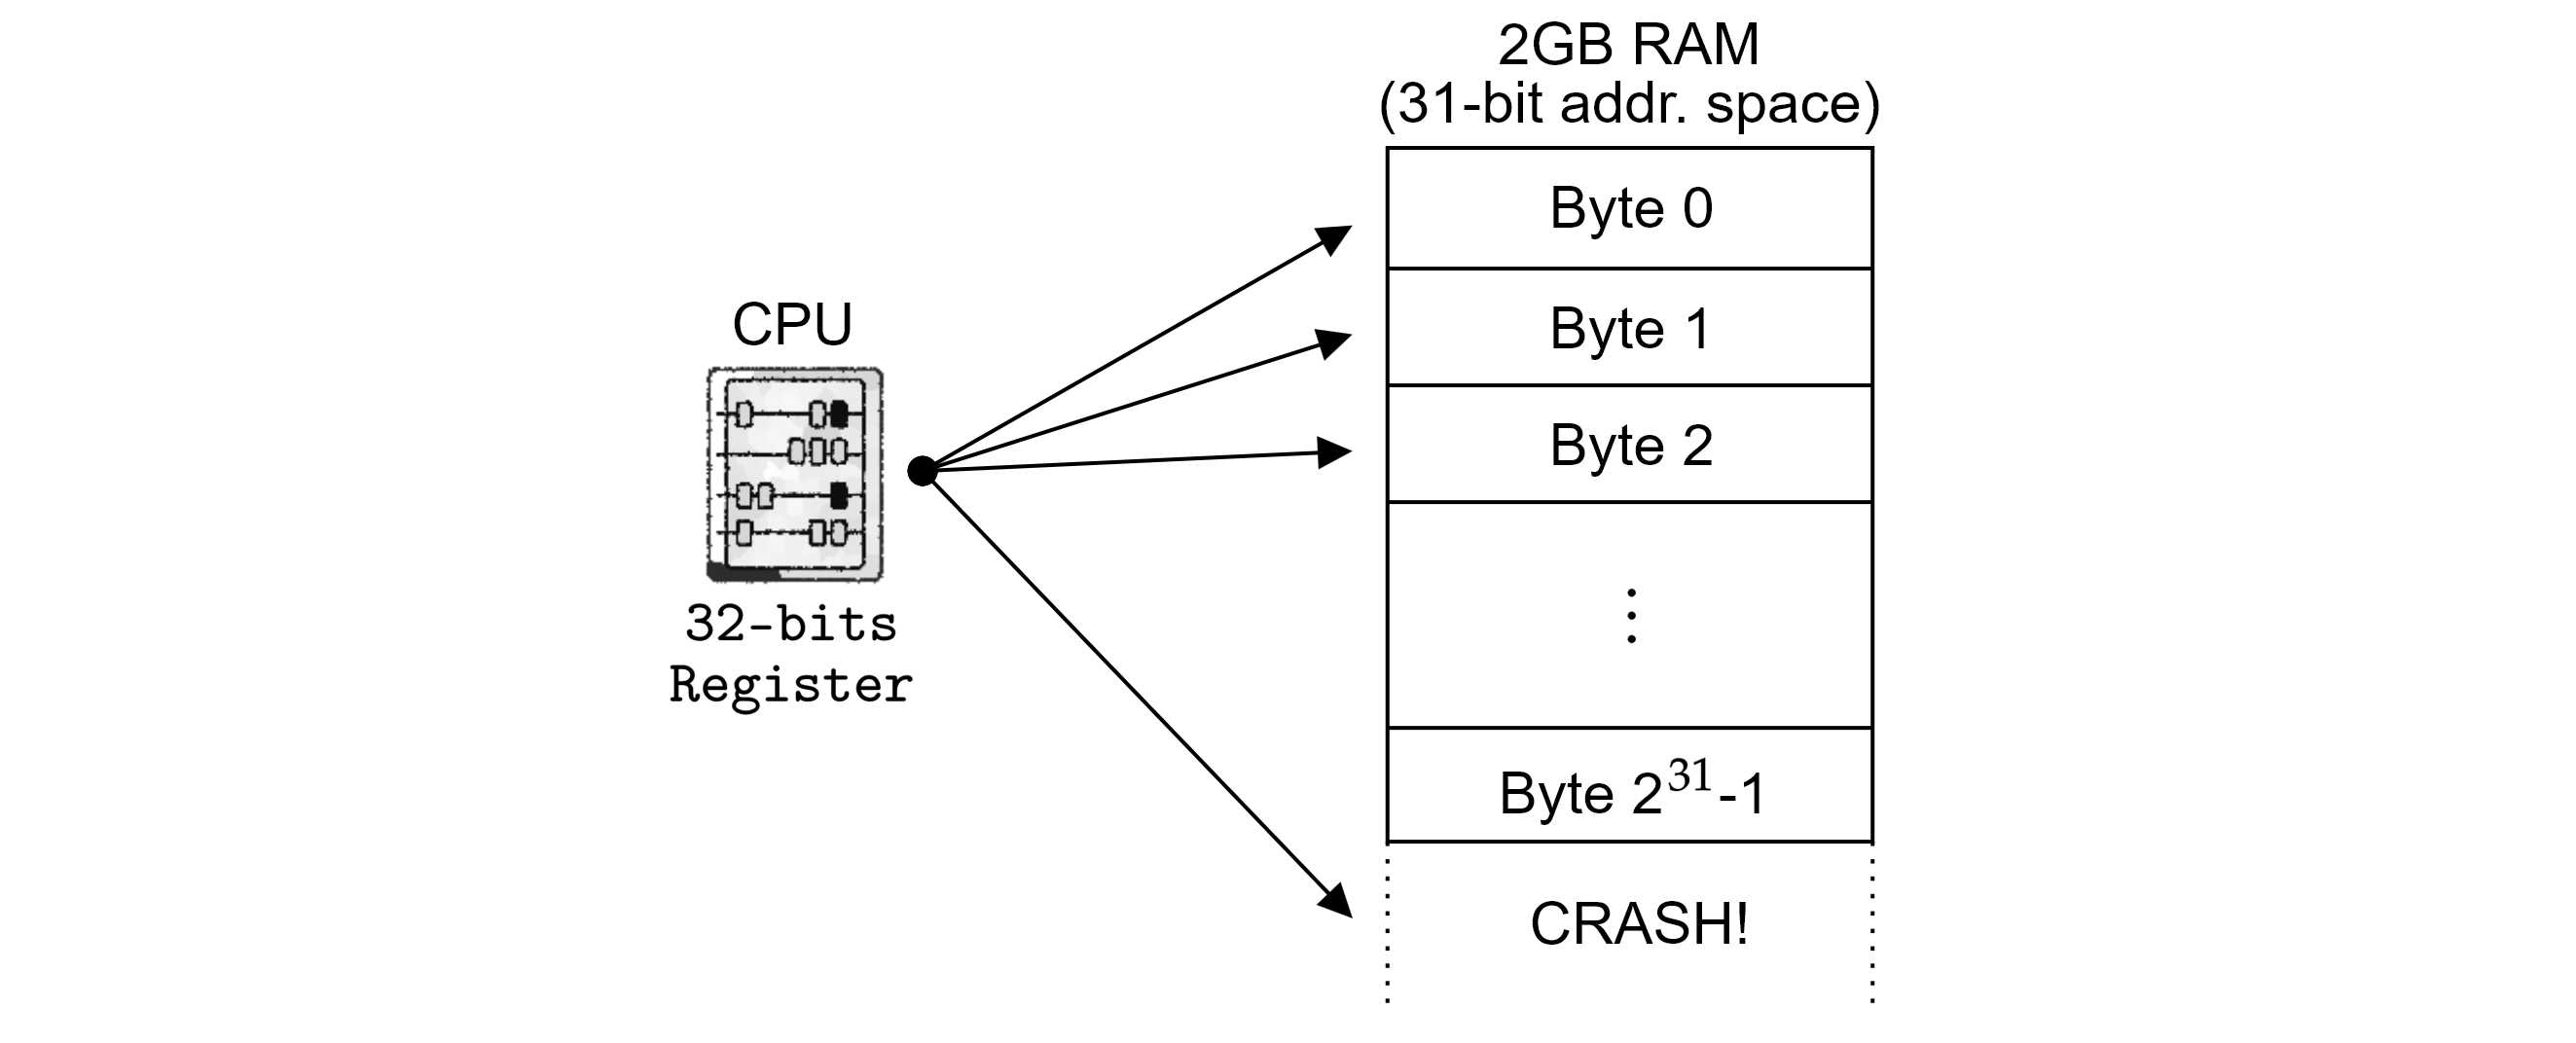
\includegraphics[width=\textwidth]{Sections/virt/crash.png}
    
    \vspace{1em}
    \caption{A 32-bit CPU accessing 2 GBs of RAM, where a crash happens when trying to access beyond the 31-bit address space.}
    
    \label{fig:virt1}
\end{figure}
\newpage 

\noindent
The next problem deals with multiple processes allocating and deallocating memory:

\begin{Def}[Memory Fragmentation]
    
    Memory can be thought of as a big array, where each cell is a resource a program can use.
    We want memory usage to be contiguous (i.e., no gaps or holes). So say we have an array 
    $$[O, O, O, O]$$

    \noindent
    Where $O$ represents free space in our array, each cell 1 GB of space. If we have processes $A$ and $B$ take 1 and 2 GBs respectively, we might have a memory layout of:
    $$[A, B, B, O,]$$

    \noindent
    If we then free process $A$, we might have a memory layout of:
    $$[O, B, B, O]$$
    \noindent
    Now, if another process $C$ needs 2 GBs of memory, it will not be able to find a contiguous space of 2 GBs, even though we have 2 GBs of free space.
    This is called \textbf{memory fragmentation}.
\end{Def}

\noindent
Now finally we have the problem of protecting memory from other processes:

\begin{Def}[Memory Security]

    In a multi-process system, processes may have collisions when trying to access the same memory space.
    For example, if process $A$ is a weather service and process $B$ is some finance service, we don't want 
    the weather service to overwrite the same memory space where the finance service is storing critical data.
    This is called \textbf{memory security}.
\end{Def}

\noindent
So in theory we want to give each process it s own portion of memory, to solve overlapping access:
\begin{Def}[Virtual Memory]

    To solve process memory collisions, we give each process its own fictional view of memory, called \textbf{virtual memory}.
    Though for this to work, each virtual view is mapped to an actual place in the original memory we call \textbf{physical memory}.\\

    \noindent
    \textbf{Virtual and physical addresses} are the cells spaces themselves.
\end{Def}

\newpage 

\noindent
Consider the figure below showing how virtual memory works in theory:

\begin{figure}[h]
    \centering
    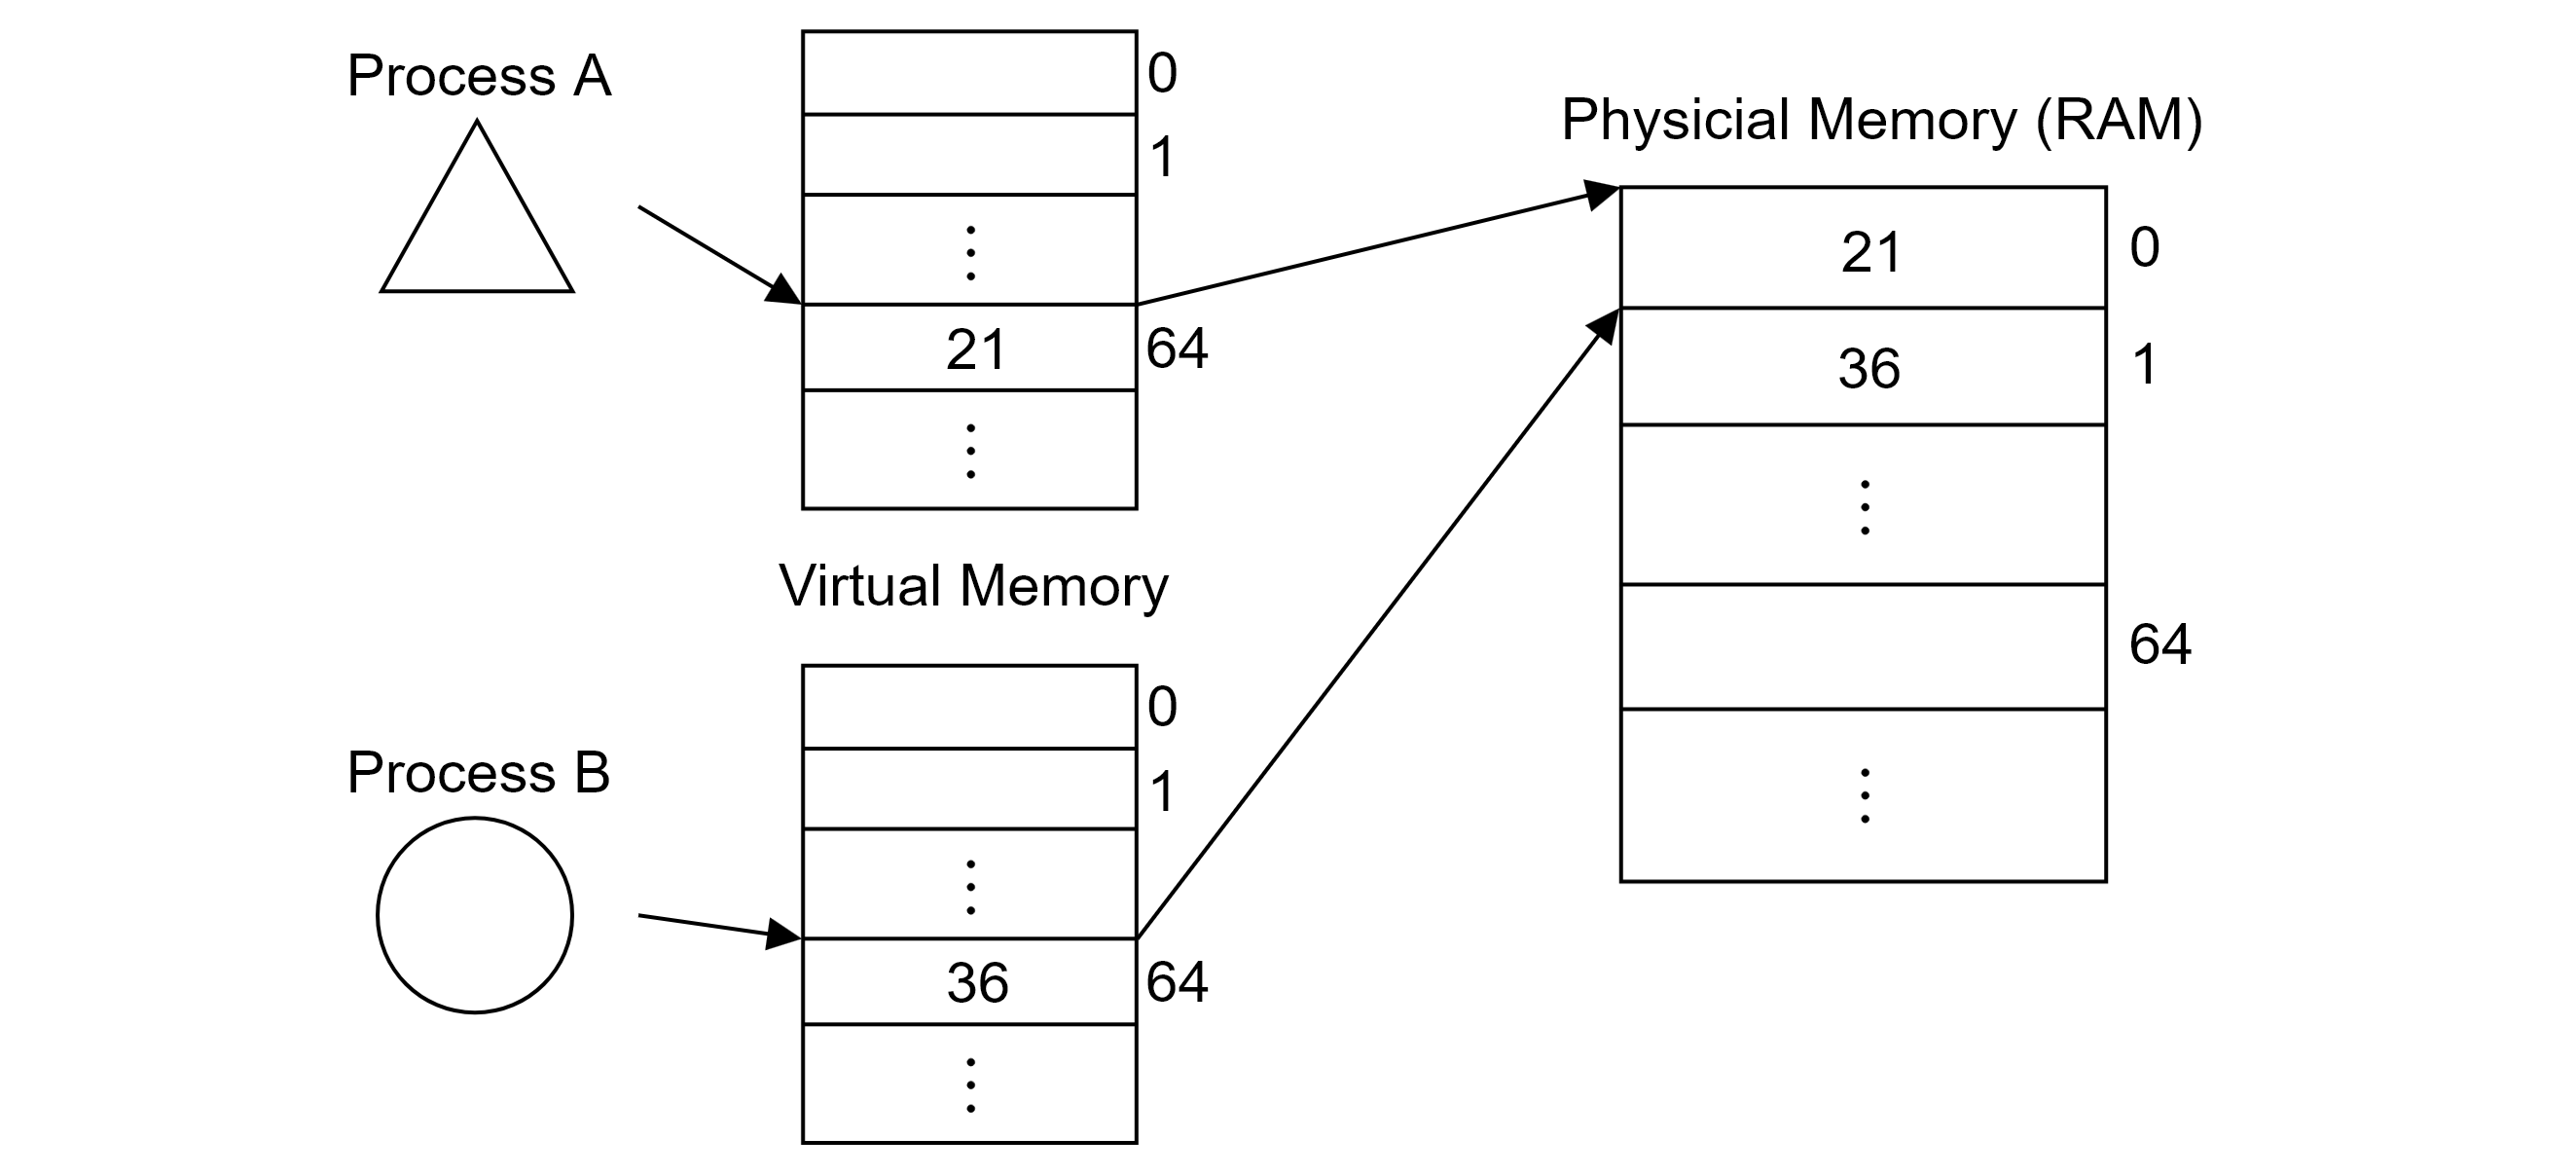
\includegraphics[width=\textwidth]{Sections/virt/virt.png}
    
    \vspace{1em}
    \caption{Processes $A$ and $B$ write to memory cell $64$ in their view of memory, but in reality they map 
    to different physical memory cells (0 and 1 respectively).}
    
    \label{fig:virt2}
\end{figure}

\noindent
A quick aside:

\begin{theo}[Physical Memory the CPU Accesses]

    In reality the CPU can access the physical memory of many other devices (e.g., hard drives, SSDs, etc.). In 
    addition, the OS takes up some of the physical memory as well. The rest is left to programs to use. The 
    program allocated space is the memory we refer to going forward as the \textbf{physical memory}.
\end{theo}

\noindent
Virtual memory solves the three problems we mentioned before:
\begin{Def}[Virtual Memory \& Not Enough Memory (Swapping)]

    The physical memory can be much smaller than what a program thinks it has in virtual memory. When a program tries to access memory 
    it does not have, the OS will \textbf{swap} physical memory to external storage to free up space. This means, while a program is not using 
    a portion of memory at a given time, the OS can swap it in and out depending on system needs.
\end{Def}

\newpage
\begin{Def}[Virtual Memory \& Fragmentation]

    Virtual memory allows programs to think they have contiguous memory. This simplifies their 
    memory management, while in reality the OS manages the split memory mappings.
\end{Def}